\documentclass[12pt,a4paper]{article}


\usepackage[in, plain]{fullpage}
\usepackage{array}
\usepackage{../pas-math}

%-------------------------------------------------------------------------------
%          -Packages nécessaires pour écrire en Français et en UTF8-
%-------------------------------------------------------------------------------
\usepackage[utf8]{inputenc}
\usepackage[frenchb]{babel}
\usepackage[T1]{fontenc}
\usepackage{lmodern}
\usepackage{textcomp}



%-------------------------------------------------------------------------------

%-------------------------------------------------------------------------------
%                          -Outils de mise en forme-
%-------------------------------------------------------------------------------
\usepackage{hyperref}
\hypersetup{pdfstartview=XYZ}
%\usepackage{enumerate}
\usepackage{graphicx}
\usepackage{multicol}
\usepackage{tabularx}
\usepackage{multirow}


\usepackage{anysize} %%pour pouvoir mettre les marges qu'on veut
%\marginsize{2.5cm}{2.5cm}{2.5cm}{2.5cm}

\usepackage{indentfirst} %%pour que les premier paragraphes soient aussi indentés
\usepackage{verbatim}
\usepackage{enumitem}
\usepackage[usenames,dvipsnames,svgnames,table]{xcolor}

\usepackage{variations}

%-------------------------------------------------------------------------------


%-------------------------------------------------------------------------------
%                  -Nécessaires pour écrire des mathématiques-
%-------------------------------------------------------------------------------
\usepackage{amsfonts}
\usepackage{amssymb}
\usepackage{amsmath}
\usepackage{amsthm}
\usepackage{tikz}
\usepackage{xlop}
%-------------------------------------------------------------------------------



%-------------------------------------------------------------------------------


%-------------------------------------------------------------------------------
%                    - Mise en forme avancée
%-------------------------------------------------------------------------------

\usepackage{ifthen}
\usepackage{ifmtarg}


\newcommand{\ifTrue}[2]{\ifthenelse{\equal{#1}{true}}{#2}{$\qquad \qquad$}}

%-------------------------------------------------------------------------------

%-------------------------------------------------------------------------------
%                     -Mise en forme d'exercices-
%-------------------------------------------------------------------------------
%\newtheoremstyle{exostyle}
%{\topsep}% espace avant
%{\topsep}% espace apres
%{}% Police utilisee par le style de thm
%{}% Indentation (vide = aucune, \parindent = indentation paragraphe)
%{\bfseries}% Police du titre de thm
%{.}% Signe de ponctuation apres le titre du thm
%{ }% Espace apres le titre du thm (\newline = linebreak)
%{\thmname{#1}\thmnumber{ #2}\thmnote{. \normalfont{\textit{#3}}}}% composants du titre du thm : \thmname = nom du thm, \thmnumber = numéro du thm, \thmnote = sous-titre du thm

%\theoremstyle{exostyle}
%\newtheorem{exercice}{Exercice}
%
%\newenvironment{questions}{
%\begin{enumerate}[\hspace{12pt}\bfseries\itshape a.]}{\end{enumerate}
%} %mettre un 1 à la place du a si on veut des numéros au lieu de lettres pour les questions 
%-------------------------------------------------------------------------------

%-------------------------------------------------------------------------------
%                    - Mise en forme de tableaux -
%-------------------------------------------------------------------------------

\renewcommand{\arraystretch}{1.7}

\setlength{\tabcolsep}{1.2cm}

%-------------------------------------------------------------------------------



%-------------------------------------------------------------------------------
%                    - Racourcis d'écriture -
%-------------------------------------------------------------------------------

% Angles orientés (couples de vecteurs)
\newcommand{\aopp}[2]{(\vec{#1}, \vec{#2})} %Les deuc vecteurs sont positifs
\newcommand{\aopn}[2]{(\vec{#1}, -\vec{#2})} %Le second vecteur est négatif
\newcommand{\aonp}[2]{(-\vec{#1}, \vec{#2})} %Le premier vecteur est négatif
\newcommand{\aonn}[2]{(-\vec{#1}, -\vec{#2})} %Les deux vecteurs sont négatifs

%Ensembles mathématiques
\newcommand{\naturels}{\mathbb{N}} %Nombres naturels
\newcommand{\relatifs}{\mathbb{Z}} %Nombres relatifs
\newcommand{\rationnels}{\mathbb{Q}} %Nombres rationnels
\newcommand{\reels}{\mathbb{R}} %Nombres réels
\newcommand{\complexes}{\mathbb{C}} %Nombres complexes


%Intégration des parenthèses aux cosinus
\newcommand{\cosP}[1]{\cos\left(#1\right)}
\newcommand{\sinP}[1]{\sin\left(#1\right)}


%Probas stats
\newcommand{\stat}{statistique}
\newcommand{\stats}{statistiques}
%-------------------------------------------------------------------------------

%-------------------------------------------------------------------------------
%                    - Mise en page -
%-------------------------------------------------------------------------------

\newcommand{\twoCol}[1]{\begin{multicols}{2}#1\end{multicols}}


\setenumerate[1]{font=\bfseries,label=\textit{\alph*})}
\setenumerate[2]{font=\bfseries,label=\arabic*)}


%-------------------------------------------------------------------------------
%                    - Elements cours -
%-------------------------------------------------------------------------------





\title{\'Equations de droites}
\date{}

\begin{document}
	
\maketitle

\section{Définition}


	Dans un repère toute droite a une équation qui peut s'écrire sous la forme :
	
	\begin{equation*}
		y \: = \: a \: x \: + \: b
	\end{equation*}
	
	Où :
	
	\begin{itemize}
		\item $a$ est le coefficient directeur (ou la pente) de la droite.
		
		\item $b$ est l'ordonnée à l'origine.
	\end{itemize}


	Un point $A$ appartient à une droite $\Delta$ si et seulement si ses coordonnées $(x_A;  y_A)$ respectent l'équation de cette droite.
\section{Montrer qu'un point appartient à une droite}

Pour monter qu'un point $A\:(x_A;  y_A)$ appartient à une droite d'équation donnée :
\begin{itemize}
	\item Dans l'équation je remplace $x$ par la valeur de $x_A$;
	\item Si la valeur que je trouve pour $y$ est la même que celle de $y_A$, alors le point $A$ appartient à la droite.
\end{itemize}

\section{Tracer une droite d'équation donnée}

\subsection{Méthode}
Pour tracer une droite il faut connaitre deux points qui appartiennent à cette droite. 

\begin{enumerate}
	\item Je choisis deux valeurs de $x$ : $x_A$ et $x_B$;
	\item Je remplace $x$ dans l'équation par chacune de ces valeurs pour obtenir $y_A$ et $y_B$;
	\item Je place dans mon repère les points $A\: (x_A; y_A)$ et $B \: (x_B; y_B)$;
	\item Je trace la droite qui passe par $A$ et par $B$
	
\end{enumerate}
Il suffit donc de choisir deux valeurs de $x$ et de calculer à l'aide de l'équation les valeurs de $y$ correspondantes. Pour ce calcul, on remplace $x$ dans l'équation par les valeurs choisies.

\newpage

\subsection{Exemple}

Je veux tracer la droite $\Delta$, d'équation $ y = 2x + 3$ :
\begin{multicols}{2}
	
\begin{enumerate}
	\item Je choisis une première valeur de $x$ : $x_A = 0$;
	\item Je remplace $x$ dans l'équation de $\Delta$ :
		\begin{eqnarray*}
			y_A &=& 2 \times x_A + 3 \\
			y_A &=& 2 \times 0 + 3 \\
			y_A &=& 0 + 3 \\
			y_A &=& 3
		\end{eqnarray*} 
	\item Je chois une deuxième valeur de $x$ : $x_B = 3$;
	\item Je calcule $y_B$, $y_B = 2 \times 3 + 3 = 9$;
	\item Je place dans le repère les points $A(0;3)$ et $B(3;9)$;
	\item Je trace la droite $(A,B)$.
\end{enumerate}

\begin{center}
	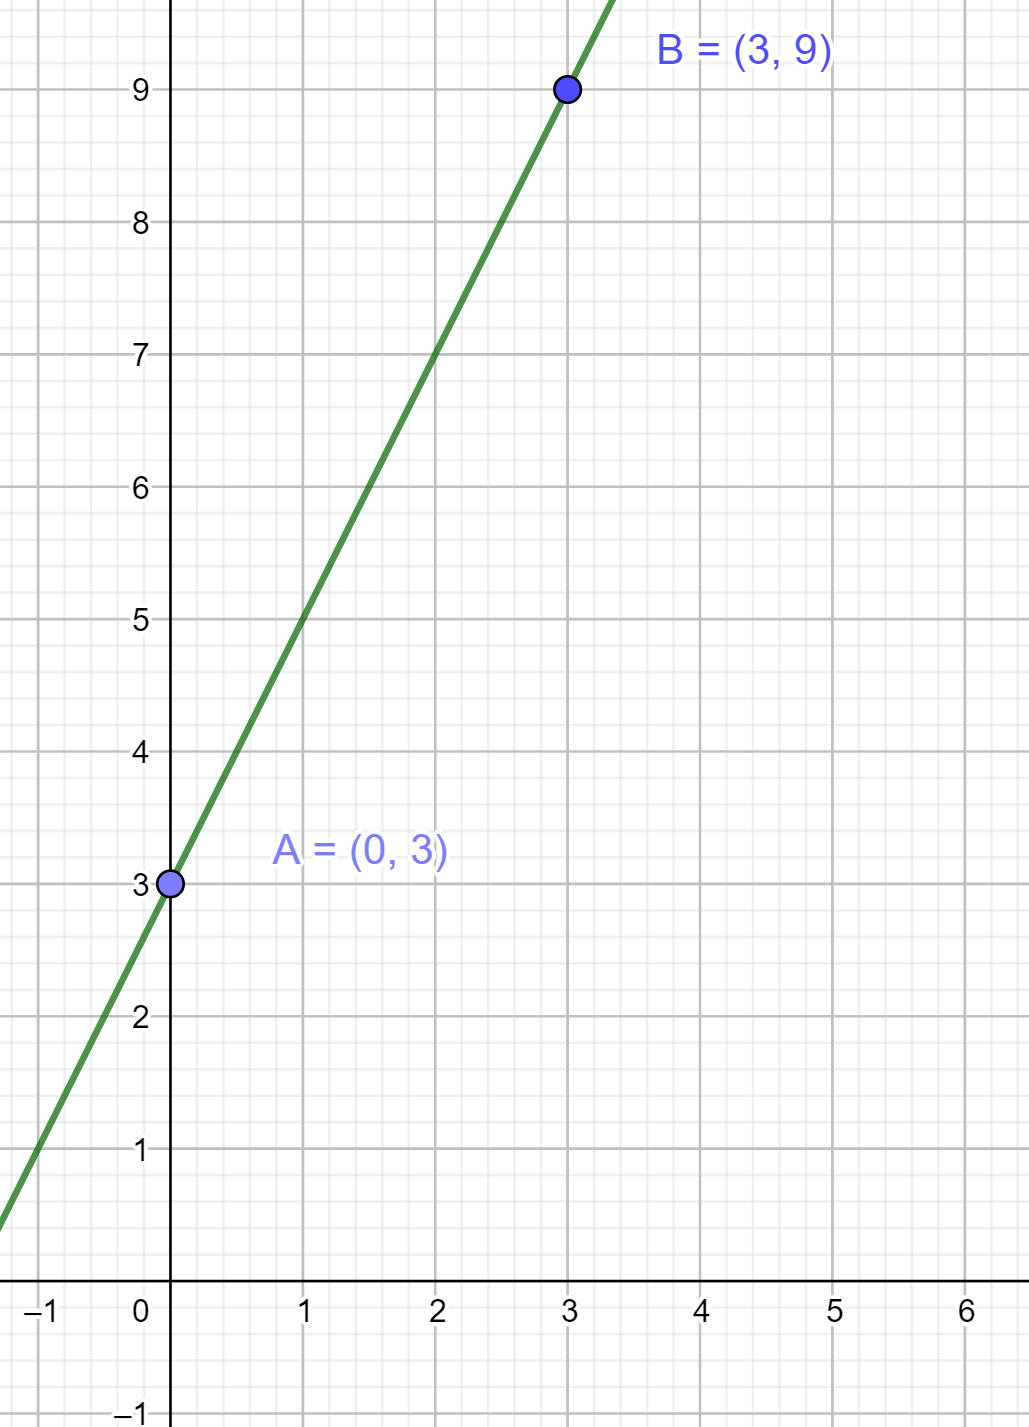
\includegraphics[scale=0.3]{img/trace_droite}
\end{center}
\end{multicols}

\section{Déterminer une équation de droite}

\subsection{Méthode}

	On détermine l'équation d'une droite à partir de deux points de cette droite $A(x_A; y_A)$ et $B(x_B; y_B)$.\\
	
	Le coefficient directeur $a$, est obtenu par le calcul suivant :
	
	\begin{align*}
	a = \dfrac{y_B - y_A}{x_B - x_A}
	\end{align*}
	
	
	L'ordonnée à l'origine $b$ est obtenue en remplaçant $x$ et $y$ dans l'équation par les coordonnées d'un des points.

\newpage

\subsection{Exemple}

	La droite $\Delta$ passe par les points $A$ et $B$ de coordonnées $(1;2)$ et $(5;4)$, on a :
	
	\begin{align*}
	a &= \frac{4-2}{5-1} \\
	a &= \frac{2}{4} \\
	a &= \num{0.5}
	\end{align*}
	
	Donc l'équation de la droite $\Delta$ est de la forme $y=\num{0.5}x+b$. Pour trouver $b$ on remplace $x$ et $y$ par les coordonnées de $A$, on a :
	
	\begin{align*}
	y &= \num{0.5}x+b \\
	2 &= \num{0.5} \times 1 + b  \\
	2 &= \num{0.5} + b\\
	\num{1.5} &= b
	\end{align*}
	
	Donc $\Delta$ est la droite d'équation $y=\num{0.5}x+\num{1.5}$.
	
	
	\begin{center}
		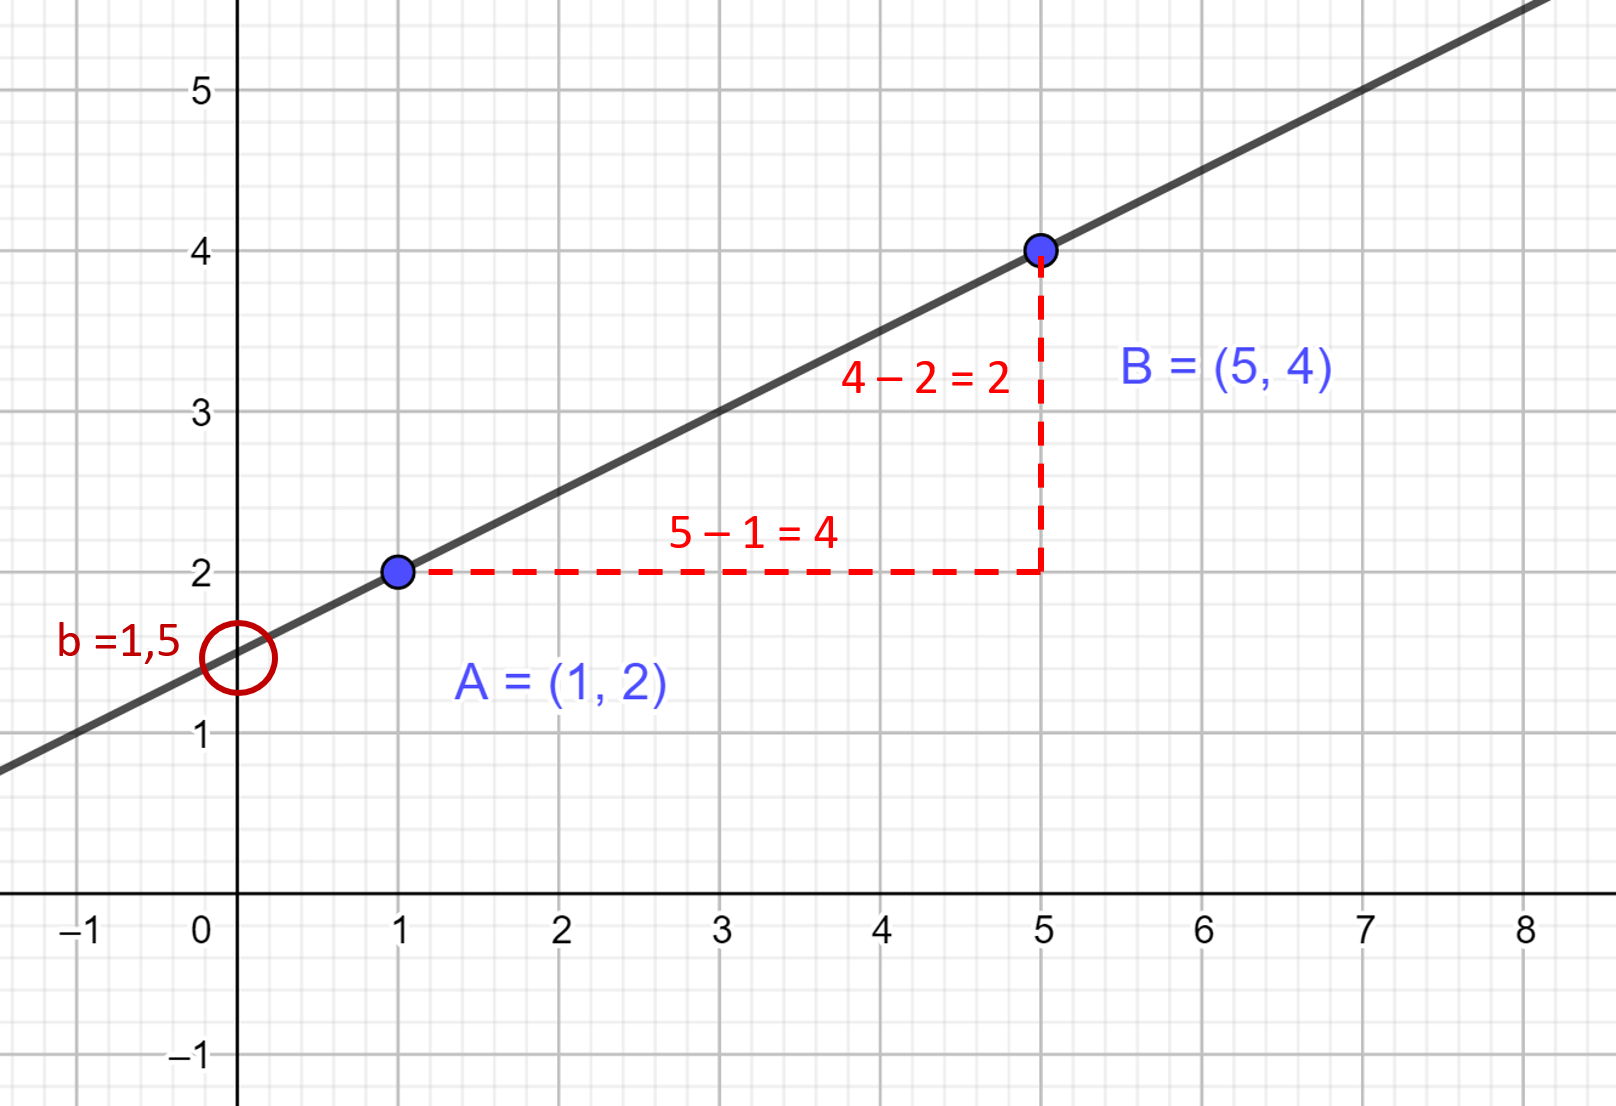
\includegraphics[scale=0.5]{img/calcul_eq2}
	\end{center}

	Remarque : On peut aussi lire l'ordonnée à l'origine à l'intersection de la droite et de l'axe des ordonnées.
	
\newpage

\section{Cas particuliers}

\subsection{Principe}
\begin{itemize}
	\item Si la droite passe par l'origine du repère, elle aura une équation du type $y=ax$.
	
	\item Si la droite est perpendiculaire à l'axe des abscisses, elle aura une équation du type $x=c$. Où $c$ est la valeur de l'intersection de la droite et l'axe des abscisses.
\end{itemize}

\subsection{Exemples}

\begin{multicols}{2}
	\begin{center}
		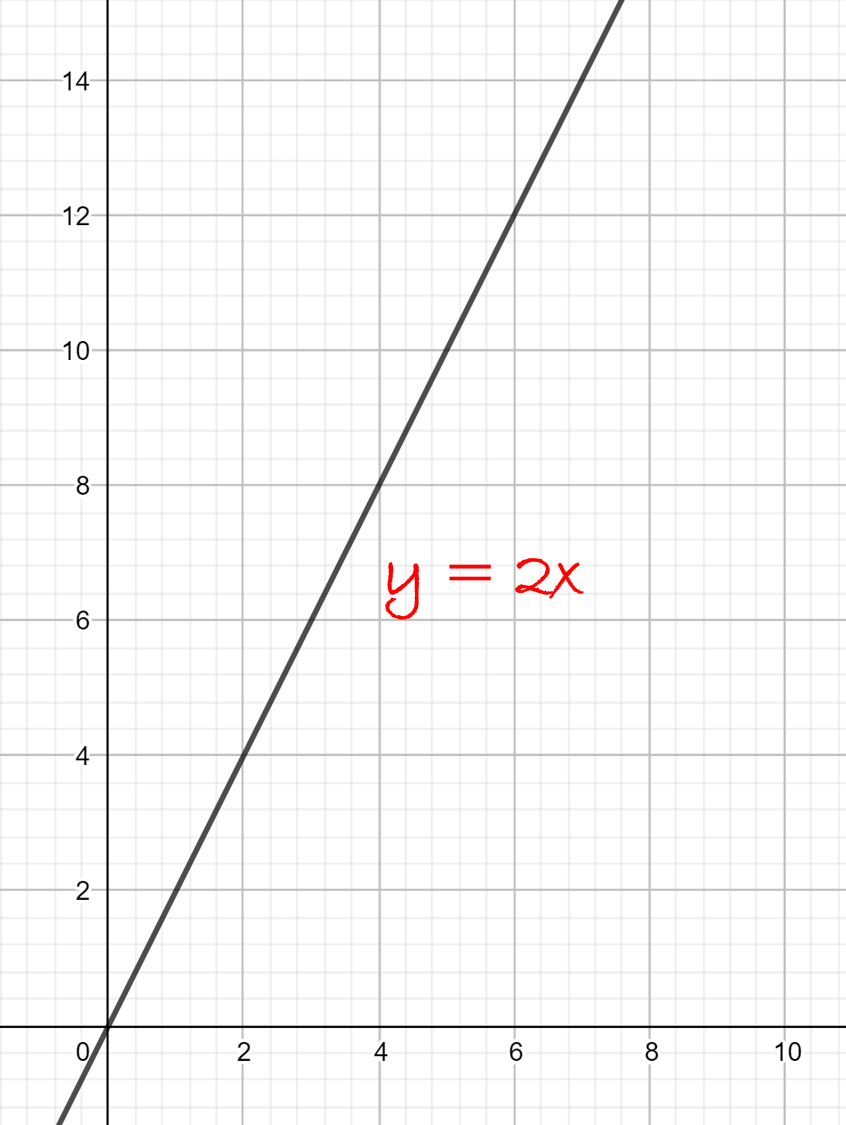
\includegraphics[scale=0.5]{img/lineaire}
	\end{center}


	\begin{center}
		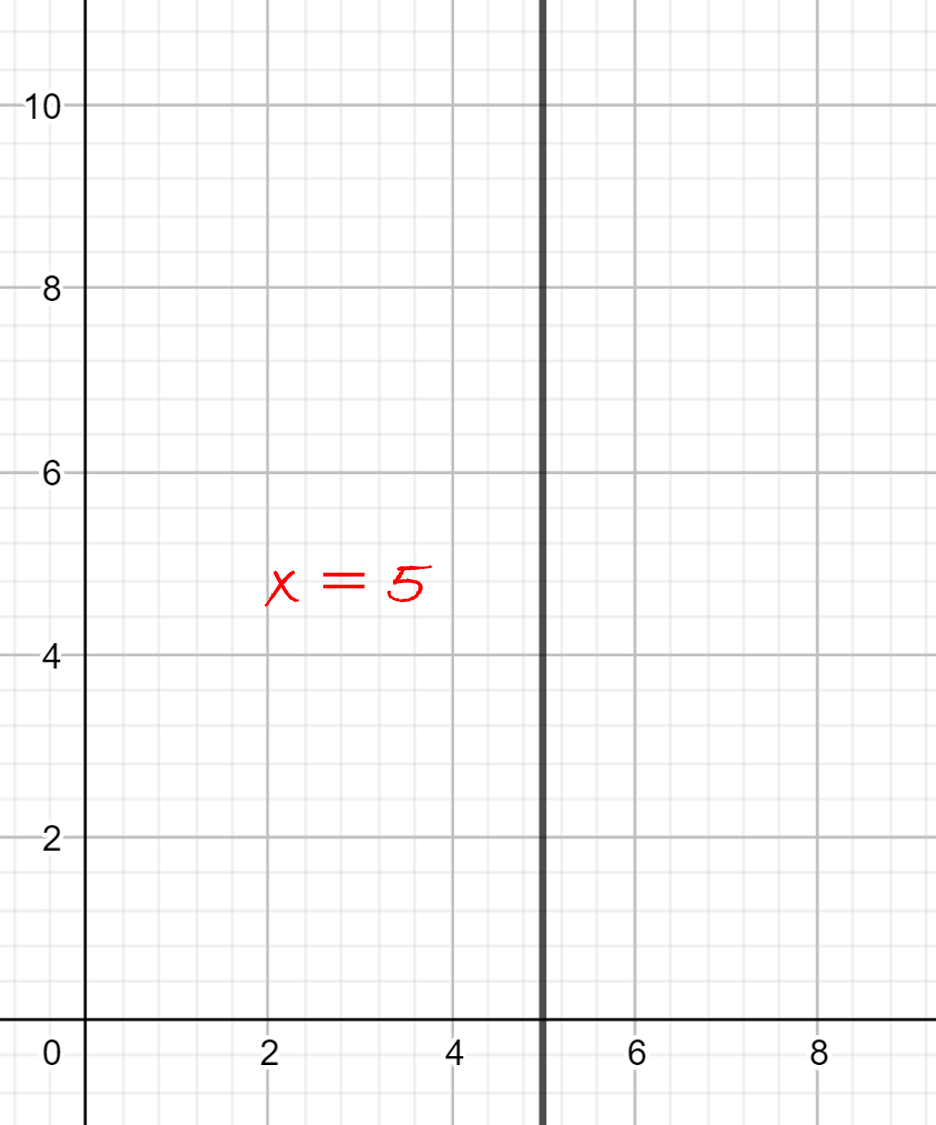
\includegraphics[scale=0.5]{img/perp}
	\end{center}
\end{multicols}
\end{document}